%
% Entanglement - The Ultimate Quantum Resource
%

\section{Entanglement -- The ultimate quantum resource} \label{sec:ent_ultimate} \index{Entanglement}

\dropcap{A}{s} we have seen, the diversity of quantum states that may be communicated, and protocols implemented over the quantum internet is extremely diverse, encompassing many different types of encodings and communications protocols.

Given this plethora of protocols and encodings, discussed in detail in Sec.~\ref{sec:protocols_quant_int}, one might ask whether there is a single primitive resource that might be applicable to all, or at least most of these quantum protocols, thereby reducing the technological requirements of the nodes and quantum channels forming the network mediating them -- if networks were able to specialise in a very limited number of tasks, we might reasonably expect them to be better optimised and exhibit better performance than a `Jack of all trades' network!

It turns out that there is one particularly useful quantum resource, that finds applicability in many of these protocols -- \textit{distributed entanglement}, which comes in many flavours and varieties, some of which we discuss now.

%
% Bell States
%

\subsection{Bell states}\index{Bell states}

Foremost, Bell pairs (Sec.~\ref{sec:bell_state_res}) -- the simplest entangled states -- are an utterly indispensable resource for countless quantum protocols. In brief, Bell pairs find applicability in, amongst many others, the following key protocols:
\begin{itemize}
\item Cluster states (Sec.~\ref{sec:CSQC})\index{Cluster states}: a Bell pair is also a 2-qubit cluster state, a supply of which can be employed in fusion strategies to prepare larger cluster states, enabling universal, distributed MBQC.
\item Quantum state teleportation (Sec.~\ref{sec:teleport})\index{Quantum state teleportation}: a shared Bell pair between Alice and Bob forms the elementary quantum resource upon which the state teleportation protocol is constructed.
\item QKD (Sec.~\ref{sec:QKD})\index{Quantum key distribution (QKD)}: the E91 QKD\index{E91 protocol} protocol is built upon a reliable stream of distributed Bell pairs, enabling private communication with perfect information theoretic security.
\item Modularised quantum computation (Sec.~\ref{sec:module})\index{Modularised quantum computation}: using Bell pairs, entanglement swapping (Sec.~\ref{sec:swapping})\index{Entanglement swapping} can be employed to fuse neighbouring, but potentially distant modules together using operations local to each module.
\item Superdense coding (Sec.~\ref{sec:superdense})\index{Superdense coding}: a shared Bell pair enables the communication of two classical bits of information via transmission of a single qubit, thereby doubling classical channel capacity\index{Channel capacity}.
\item Quantum-enabled telescopy (Sec.~\ref{sec:telescopy}): a shared Bell pair between two telescopes allows a photon received at one telescope to be teleported to the other, at which point interferometric techniques yield extremely sensitive phase information.
\end{itemize}

We see that Bell pairs form a ubiquitous resource, covering many of the most significant quantum protocols in quantum computation, distributed quantum computation, quantum state teleportation, and quantum cryptography.

%
% GHZ States
%

\subsection{GHZ states}\index{Greenberger-Horne-Zeilinger (GHZ) states}

Beyond Bell pairs, multi-qubit GHZ states\index{Greenberger-Horne-Zeilinger (GHZ) states} (Sec.~\ref{sec:GHZ_states}) (the direct generalisation of Bell pairs to $n$ qubits) are useful in a variety of settings.

For the purposes of quantum anonymous broadcasting\index{Quantum anonymous broadcasting} (Sec.~\ref{sec:anon_broad}), multi-party GHZ entanglement is the primitive resource upon which the cryptographic protocol is constructed. As with Bell pairs, GHZ states are a known state and infinitely reproducible. They can also be purified. Thus, GHZ entanglement distribution is another useful primitive, which future quantum hubs might specialise in preparing and distributing.

Additionally, quantum gate teleportation (Sec.~\ref{sec:teleport_gate})\index{Quantum gate teleportation} of a maximally-entangling 2-qubit gate (e.g a CNOT or CZ gate) is mediated via a shared 4-qubit GHZ state. In a distributed environment the sharing of such a state between two parties (2 qubits per party) enables implementation of a truly distributed 2-qubit entangling gate.

\comment{Any other uses?}

%
% Cluster States
%

\subsection{Cluster states}\index{Cluster states}

Finally, cluster states\index{Cluster states} (Sec.~\ref{sec:CSQC}) are a primitive resource for measurement-based quantum computation\index{Cluster state model}. Owing to their handy ability to fuse together to one another, forming larger clusters, the preparation and distribution of relatively small cluster states lends itself well to distributed implementation by specialised providers. Providers could distribute small cluster states, which are subsequently fused together using simple 2-qubit entangling operations to form desired topologies, held either locally or distributed in the cloud.

%
% Why Specialise in Entanglement Distribution?
%

\subsection{Why specialise in entanglement distribution?}

These observations warrant special treatment of entanglement distribution as a fundamental building block in the quantum era. One might envisage a quantum internet in which a central server(s), who specialises in only entangled state preparation and distribution, serves the sole role of pumping out Bell pairs or other entangled states across the quantum internet to whomever requests them, who subsequently use them for protocols such as those mentioned above. This could be in the form of a server transmitting over fibre networks, across free-space, or via a satellite in orbit, transmitting at an intercontinental level.

What's the advantage of this approach to quantum networking? Why specialise in entanglement distribution, rather than implementing more capable networks with the ability to perform arbitrary operations? There are numerous:
\begin{enumerate}
\item Dedicated servers can specialise in this one particular task, as can be the transmission infrastructure.
\item The entanglement servers are entirely passive, not involved interactively with clients.
\item The server needn't concern itself with the nitty-gritty of the protocols implemented by the end-user. It acts purely as a provider of a single resource, remaining uninvolved in their subsequent applications.
\item Because servers are providing a single standardised product, they can be commodified, enabling mass production of the hardware devices and the associated economy of scale. For example, mass production of simple ground-based Bell state relays, or the construction of a comprehensive globe-enveloping constellation of satellites, would inevitably improve economies of scale.
\item Unlike generic quantum states, Bell pairs, GHZ states and cluster states are known states that are infinitely reproducible, without having to worry about no-cloning\index{No-cloning theorem} limitations.
\item Photonic Bell pairs are easily prepared via type-II SPDC at very high repetition rates (\mbox{$\sim 100$MHz-1GHz}), enabling rapid state preparation.
\item Small entangled states like Bell pairs are relatively `cheap' to prepare, and can be readily manufactured using widely accessible, present-day technology that has already been well-demonstrated on Earth and in space \cite{???}.
\item QoS is a lesser issue in most scenarios. We can employ a \textsc{Send-and-forget}\index{Send-and-forget strategy} protocol for the distribution of entanglement (much like classical UDP\index{User Datagram Protocol (UDP)}) -- since every state is identical, we needn't be concerned about missing ones. Instead, we can simply wait for the next one (a \textsc{Repeat-until-success}\index{Repeat-until-success strategy} strategy), knowing it will be exactly the same. We also call this the \textsc{Shotgun}\index{Shotgun state preparation} approach -- keep firing away until we hit something, and if we lose a few, who cares?
\item Rather than transmitting quantum states between distant parties directly, if we instead use state teleportation (Sec.~\ref{sec:teleport}) mediated by Bell states, the state to be transmitted will not be corrupted if the communications channel fails (e.g via loss). Instead we can wait for the next successfully transmitted Bell pair until we are ready to teleport the state, which then proceeds without directly utilising the quantum communications channel, accumulating its associated costs, or risking losing the state altogether should link failure occur. Only classical communication is required to complete the protocol, which can be regarded as error-free for all intents and purposes.
\item Entanglement purification may be employed by parties to improve the cost metrics associated with their shared entanglement, thereby partially overcoming the limitations imposed by the quantum communication channels.
\item If no direct link exists between server and clients, bootstrapped entanglement swapping can be employed to concatenate servers to create longer-distance `virtual' links. This is the basis for \textit{quantum repeater networks}, to be discussed next in Sec.~\ref{sec:rep_net}.
\end{enumerate}

\comment{Any other advantages?}

%
% Why Not Distributed Entangling Measurements
%

\subsection{Why not distributed entangling measurements?}

In addition to entanglement distribution, entangling measurements, e.g Bell state projections (Sec.~\ref{sec:bell_proj}), may be used as a primitive for many protocols. This is effectively entangled state distribution in reverse\index{Distributed entangling measurements}, whereby two clients transmit states to a host, who performs a joint entangling measurement upon them. For example, in the modularised model for cluster state quantum computing\index{Cluster state model}, two adjacent but distant modules might transmit optical qubits to a satellite, which projects them into the Bell basis, thereby creating a link between the respective modules via entanglement swapping\index{Entanglement swapping}. This isn't as powerful as entangled state distribution, since it cannot be used for, for example, E91 QKD\index{E91 protocol}, but nonetheless remains a powerful primitive for many protocols.

So which ought our quantum hubs specialise in, entanglement distribution, entangling measurements, or both? For most practical purposes the former is far more powerful and robust. Let us take the example of fusing two remote cluster states together to form a larger, distributed virtual cluster. Imagine that their fusion operations are optically mediated by a satellite overhead. The options for satellite-mediated state fusion are (see Fig.~\ref{fig:sat_up_down}):
\begin{itemize}
	\item Downlink mode\index{Satellite downlink} --- The satellite uses the downlink to distribute an entangled Bell pair between the two nodes. Each node performs a Bell projection between their half of the Bell pair and their respective qubit from their local cluster state, thereby swapping the entanglement and creating a link.
	\item Uplink mode\index{Satellite uplink} --- Each node takes an optical qubit from their cluster state (or entangles their cluster state qubit with an optical qubit), which is uplinked to the satellite. The satellite performs a Bell projection between the two received optical qubits, thereby implementing entanglement swapping between the two nodes, creating a link.
\end{itemize}

\if 2\pubmode
	\begin{figure}[!htbp]
		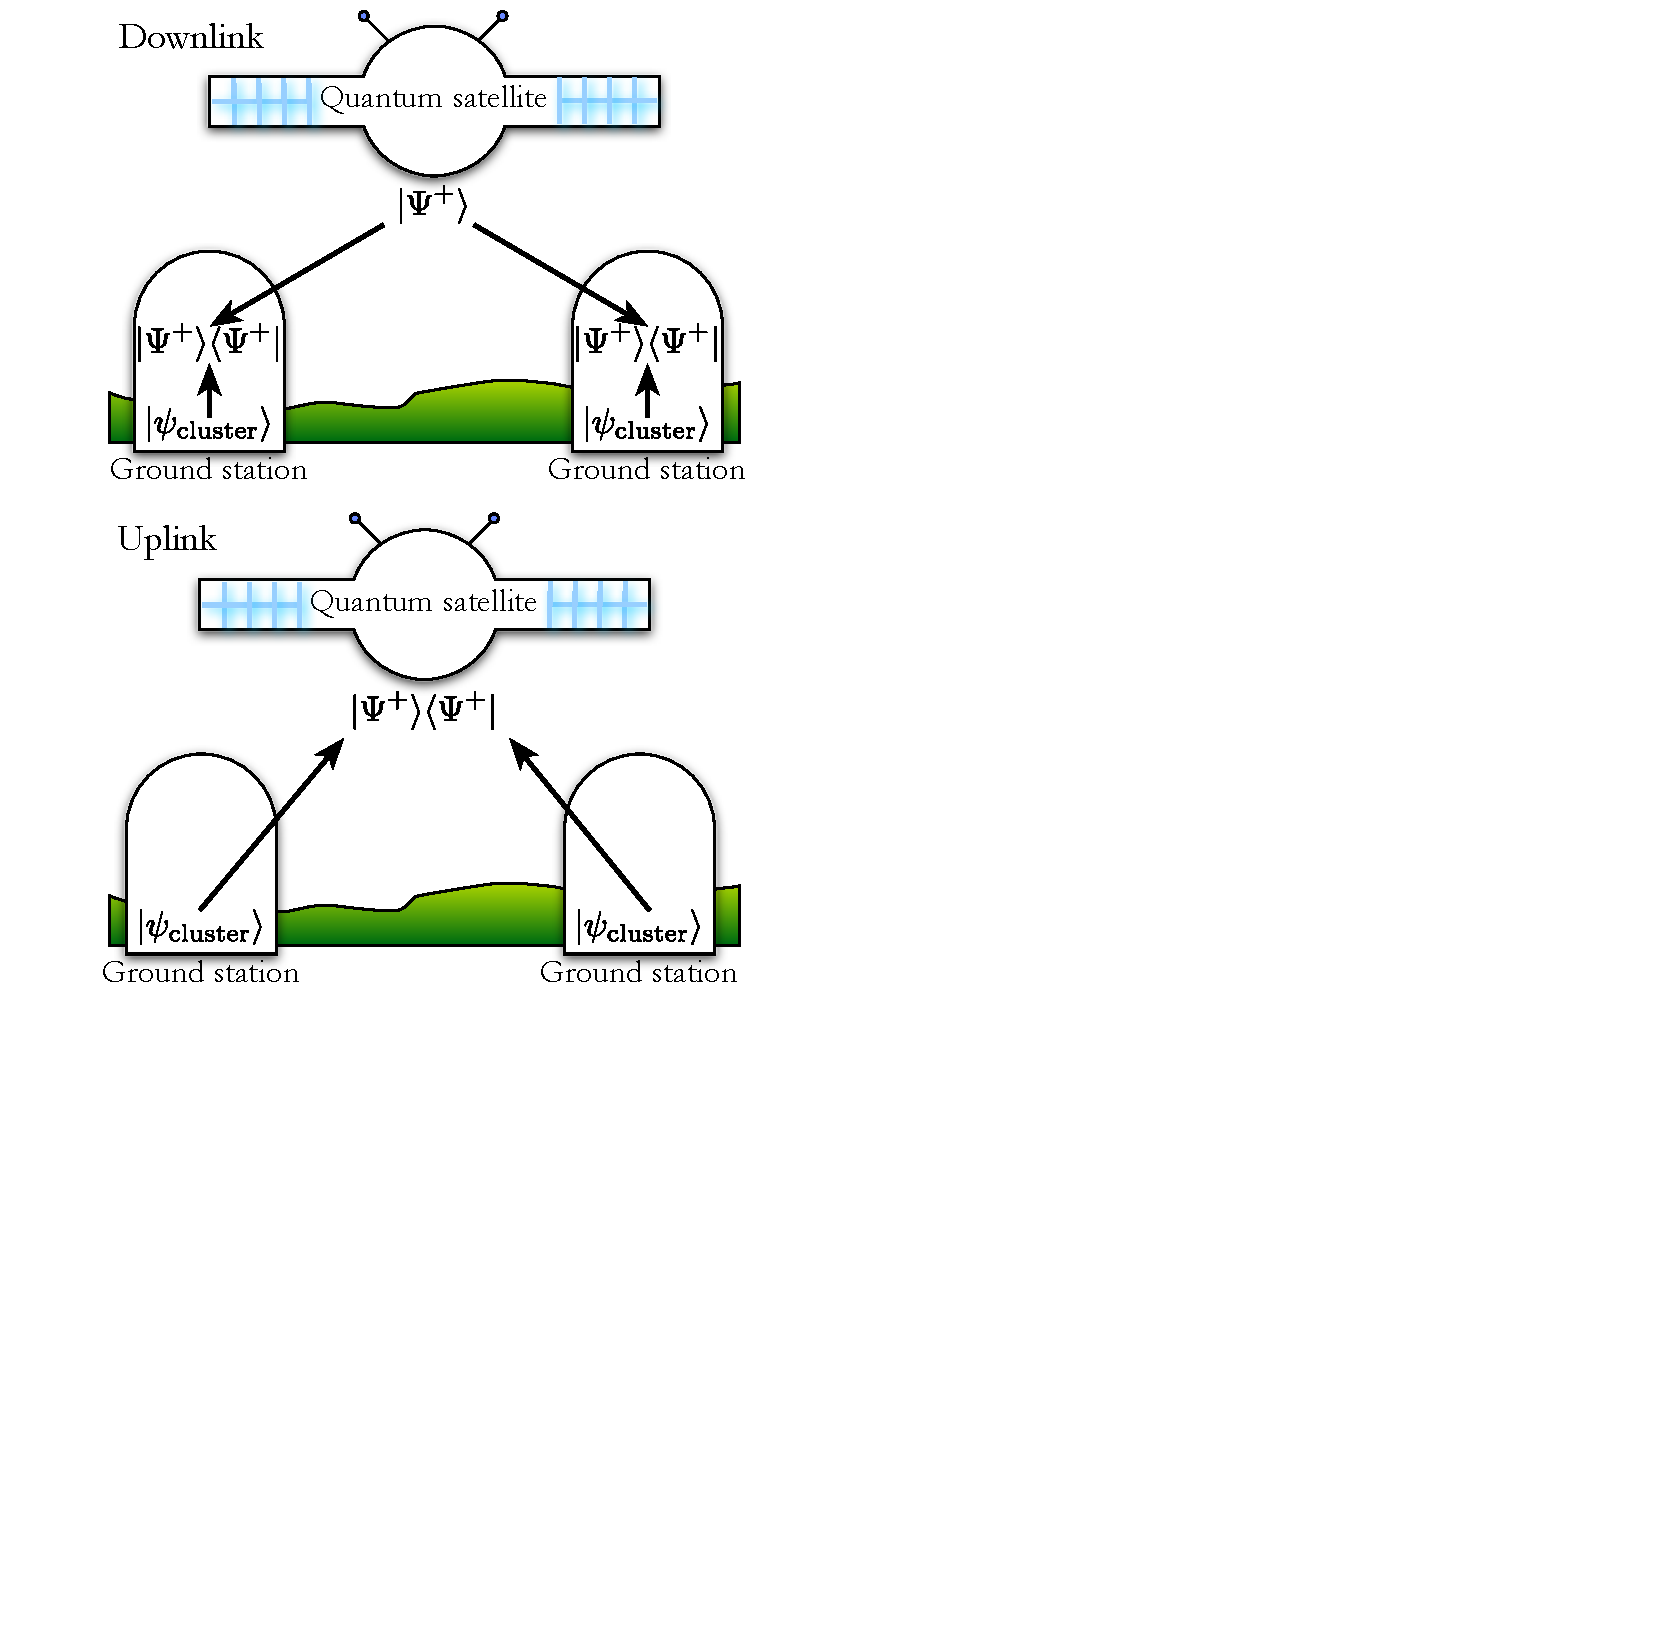
\includegraphics[clip=true, width=0.475\textwidth]{satellite_downlink_uplink_long}
		\captionspacefig \caption{Satellite-mediated cluster state fusion operations for creating a link between two cluster states held by distant ground nodes. (top) Via entanglement distribution over a downlink channel. (bottom) Via distributed Bell projection over an uplink channel. When performing a distributed Bell measurement it is essential that the optical qubits arrive synchronously at the entangling measurement device, denoted \mbox{$\ket{\Psi^+}\bra{\Psi^+}$} (e.g a PBS), which is technologically challenging to implement on satellite given the unpredictable nature of the atmospheric quantum channel, necessitating on-board quantum memories to synchronise the qubits. This is likely to make downlinks cheaper, faster and more efficient than uplinks.} \label{fig:sat_up_down}
	\end{figure}
\else
	\begin{figure*}[!htbp]
		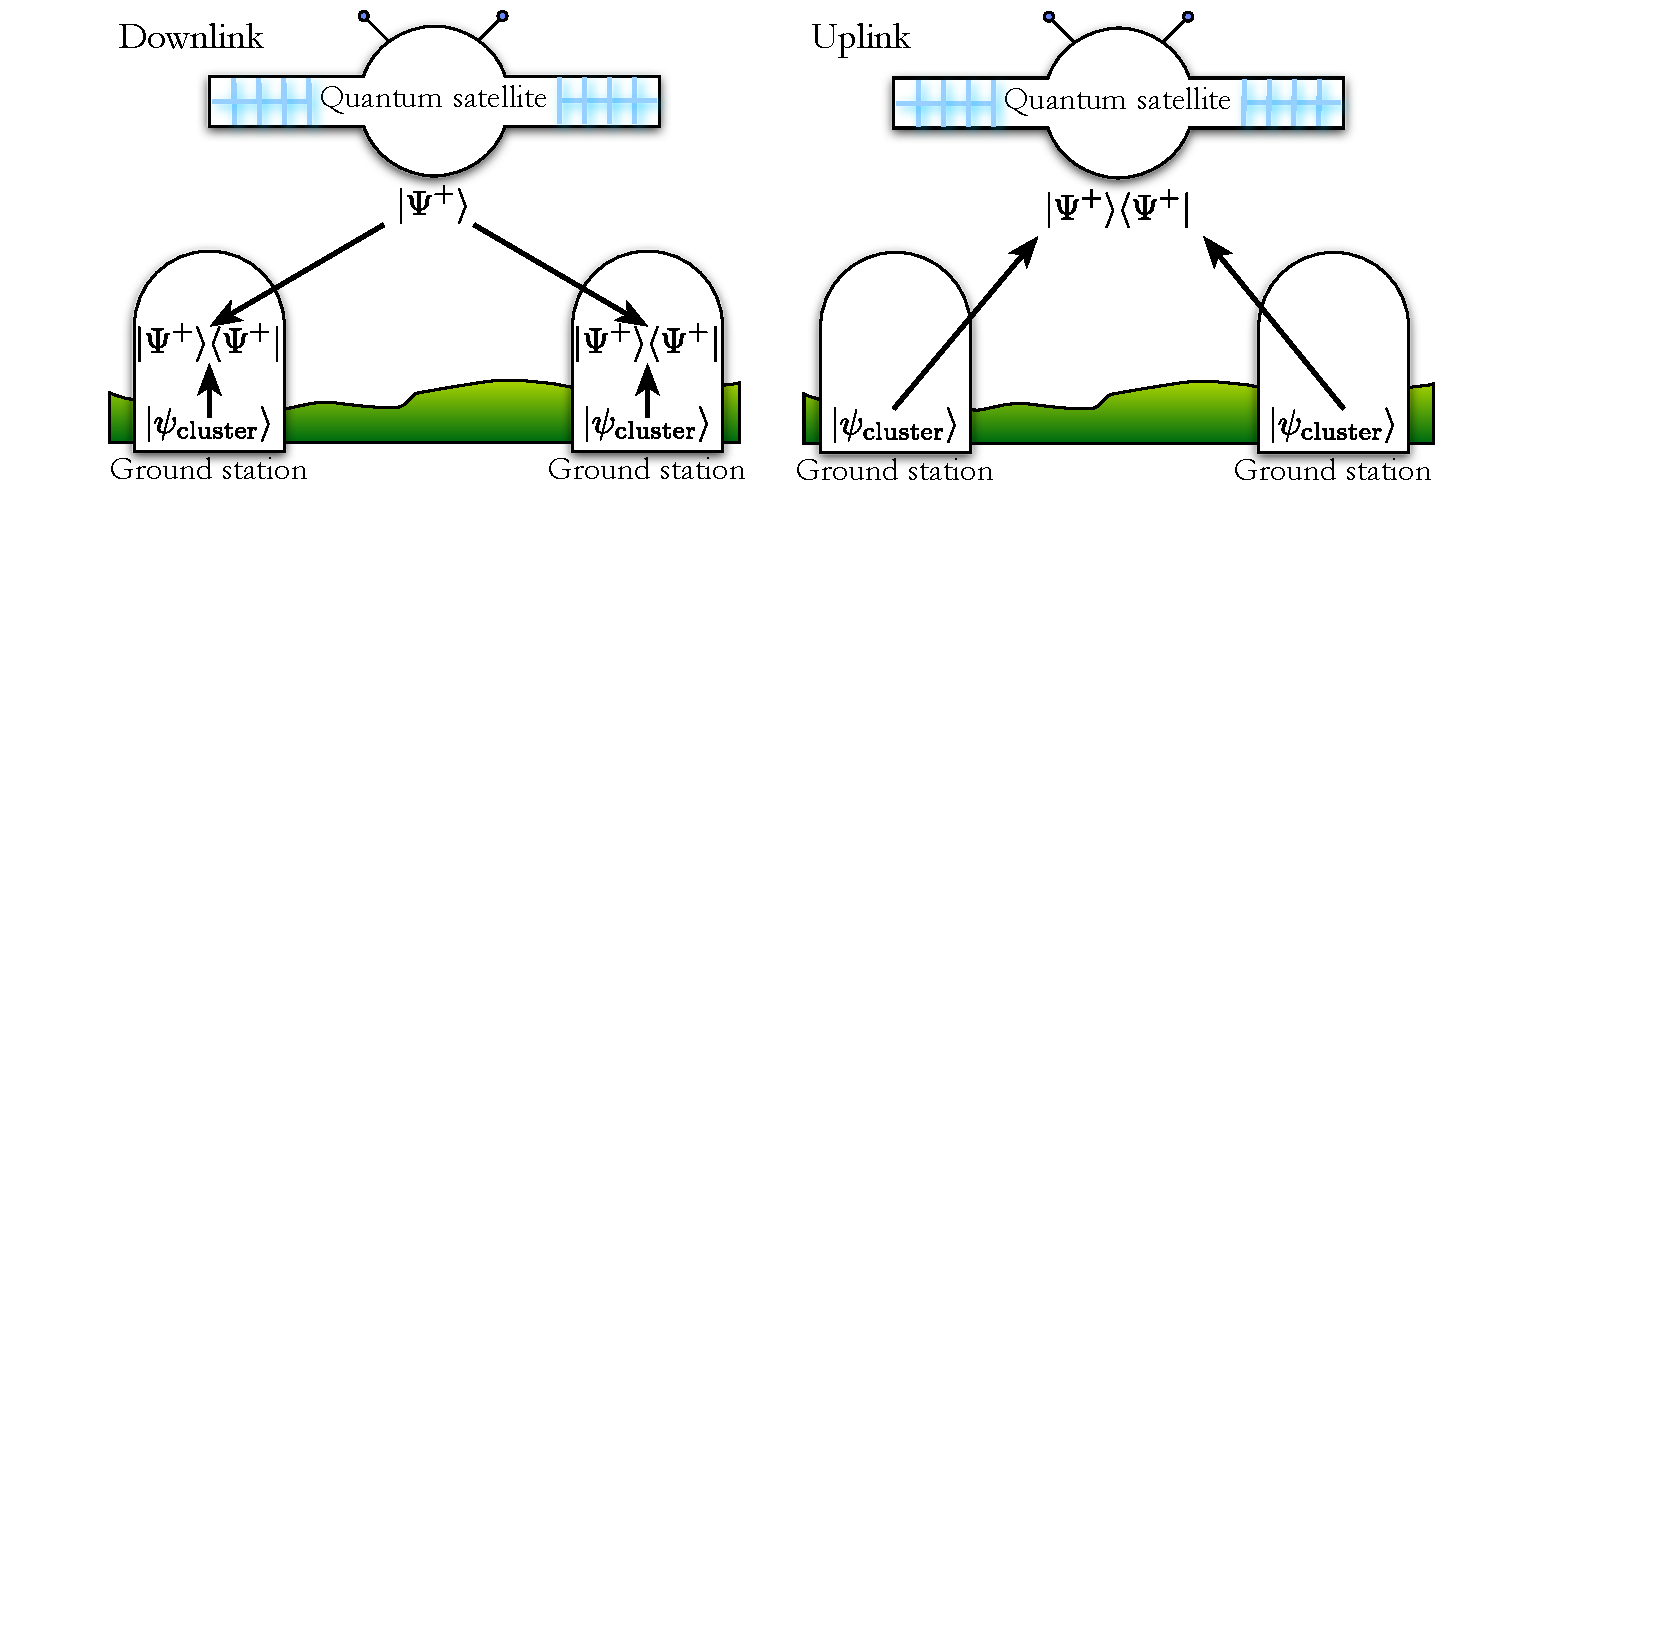
\includegraphics[clip=true, width=\textwidth]{satellite_downlink_uplink}
		\captionspacefig \caption{Satellite-mediated cluster state fusion operations for creating a link between two cluster states held by distant ground nodes. (left) Via entanglement distribution over a downlink channel. (right) Via distributed Bell projection over an uplink channel. When performing a distributed Bell measurement it is essential that the optical qubits arrive synchronously at the entangling measurement device, denoted \mbox{$\ket{\Psi^+}\bra{\Psi^+}$} (e.g a PBS), which is technologically challenging to implement on satellite given the unpredictable nature of the atmospheric quantum channel, necessitating on-board quantum memories to synchronise the qubits. This is likely to make downlinks cheaper, faster and more efficient than uplinks.} \label{fig:sat_up_down}
	\end{figure*}
\fi

Mathematically, these two processes are almost identical in their operation, differing only in direction. However, the former has the key advantage that it requires no time-synchronisation operations on the server side, whereas the latter does, and satellite-based hardware is orders of magnitude more expensive than Earth-based hardware.

Both scenarios involve Bell projections. These entangling measurements require active synchronisation to ensure that the measured qubits arrive at the entangling measurement device (typically a PBS) simultaneously, so as to achieve high HOM-visibility\index{HOM-visibility}, requiring synchronisation on the order of the photons' coherence length\index{Coherence length}. This can be achieved either using a brute-force \textsc{Repeat-Until-Success} mode of operation (post-selecting on events where both qubits arrive within a required temporal window), or storing one qubit in quantum memory\index{Quantum memory} until the other arrives. However, post-selection is expensive, requiring a massive overhead in the number of trials, and quantum memory is technologically challenging to implement, more so in space.

In the former case, the time ordering of the Bell projections performed locally on the ground nodes is irrelevant. Although within each ground station the two qubits being projected must be synchronised, requiring quantum memories within ground stations.

On the other hand, in the latter case it is essential that both optical qubits arrive at the satellite's entangling measurement device simultaneously, which is extremely difficult to enforce when our quantum channels are tracking moving targets in low-Earth orbit and traversing a turbulent atmospheric channel in between. An on-satellite quantum memory would be extremely costly!

This yields several key advantages in favour of entanglement distribution as opposed to server-side joint entangling measurements:
\begin{enumerate}
	\item The challenging prospect of quantum memory may operate on Earth, far less onerous and expensive than incorporating this technology into a satellite in low-Earth orbit.
	\item Because the server is not storing any qubits in quantum memory, it does not suffer downtime associated with the periods between receiving the first photon and waiting for the second -- it can continue to spit out Bell pairs at maximum capacity.
	\item The satellite remains passive, implementing only the simplest of possible operations, reducing mass-production costs.
	\item The satellite does not require any interaction with its clients (classical or quantum).
	\item Because Bell pairs are known, infinitely reproducible states, the server can operate in a UDP-like\index{User Datagram Protocol (UDP)} mode and it is not problematic if any given pair was lost. In the reverse direction, loss of a qubit could compromise the entire peripheral state associated with it in the ground statio.
	\item Entanglement purification can be employed to enhance the effective quality of the transmission channel.
\end{enumerate}

We therefore anticipate that distributed entangling operations are likely to be mediated via entanglement distribution rather than distributed entangling measurements in the future quantum internet.

These observations lead us to naturally conclude that a quantum network specialised to this one particular task -- entanglement distribution -- would already be immensely useful, and on its own enable many key applications.